\documentclass[runningheads,a4paper]{llncs}

\usepackage[utf8]{inputenc}
\usepackage{graphicx}
\usepackage{listings, color}
\usepackage[bookmarks,bookmarksopen,bookmarksdepth=2]{hyperref}

\graphicspath{ {./img/} }

%% CUSTOM BINDINGS %%

\usepackage{amsmath}

 
\usepackage{alltt}
\newcommand{\TODO}[1]{\begin{alltt}\textcolor{magenta}{TODO: #1}\end{alltt}}

\newenvironment{LGContent}
{ \par\color{blue} \it \small }
{ \par }

\usepackage{verbatim}
% Use this to hide text in TODO commands and LGContent environments.
%\renewcommand{\TODO}[1]{}
%\renewenvironment{LGContent}{ \comment  }{ }
\newenvironment{LGContent-Hidden}{ \comment  }{ }

\usepackage{xspace}
\newcommand{\om}{[...]\xspace} % omission

\authorrunning{H. Hartmann, T. Wambach, M. Meffert, R. Grimm}

%% END CUSTOM BINDINGS %%

\begin{document}

%============================================================

\title{Privacy Analysis of a Mobile Sensor Application}
\author{Heinrich Hartmann \and Tim Wambach \and Maximilian Meffert \and R\"udiger Grimm}
\institute{University of Koblenz-Landau}
\maketitle

%============================================================

\begin{abstract}

\TODO{(later)}

\keywords{
privacy protection, IT security analysis, sensor data, mobile phones, traffic survey
}

\end{abstract}

%============================================================

\section{Introduction}

\TODO{RG\\
* Context: Reference model IT Security analysis\\
* Application: Travel Survey\\
* Different definitions of privacy in the literature.\\
* Study outcomes depend on privacy definition
}

\begin{LGContent}
In recent days the importance of privacy protection has been amplified
by the reports about the mass surveillance of ordinary citizens on a
global scale by the NSA and other intelligence agencies around the
world.

While aiming at the noble cause of enhancing eParticipation using
mobile technologies, Live+Gov systems do process a large variety data
that is potentially infringing the citizens privacy. The captured data
includes personal information like name, phone numbers and email
addresses and sensor data from GPS and accelerometer sensors. Also
with some applications it is possible to gather images and textual
input from the citizen.

While the collection of this data is necessary for providing the
advanced services that Live+Gov aims to deliver, at he same time, the
available raw data can be used to draw a very detailed picture of the
private life of the citizen. For instance can GPS location tracking be
used to reveal shopping habits (e.g. when a car seller is visited) and
associations to political groups (when a meeting is
attended). Accelerometer data can be used to infer medical conditions
like walking disabilities. Images can contain faces of nearby persons
to with whom the citizen is associated. All this data is highly
sensitive to the citizens privacy and can be used against the citizen
if it falls in the wrong hands.

The great importance of protecting the citizens privacy should be
apparent from these examples. The European Union, as well as many
other countries in the past, has set out a number of directives that
regulate the collection, processing and use of privacy sensitive
data. We explain the most relevant legislation in Section
\ref{sec:legal}.

The ethical aspects of privacy have been the subject of study of many
social scientists and philosophers. One scholar which is particularly
relevant in our context is Charles Fried. He investiages, why we are
intuitively so sensitive to violations of our privacy. For him privacy
is not asserted as an intrinsic value by itself, he rather sated:

\begin{quote}
Privacy is not simply an absence of information about us in the minds of others;
rather it is the control we have over information about ourselves.
\end{quote}

Fried`s study on the understanding of privacy provided a great
contribution to the research on the same term in philosophy and
computer science and despite the fact his text was published in 1970,
he already included technologies to its viewpoint (like location
monitoring) that are particularly relevant to our Context.  We explain
his theory in \ref{sec:ethics} and follow his definition of privacy in
this document.

In this document we perform a thorough analysis of how to protect the
privacy of a citizen and present several implementations that form the
core of our privacy aware Sensor Data Storage and Mining Infrastructure.

We identify six main threats for the citizens privacy, and derive
eight recommendations that should be followed in order to reduce the
associated risks for hazards.  This analysis form the guideline for
the selection of 9 measures that were implemented in our system and
documented in Chapter \ref{chap:impl}.
\end{LGContent}

%============================================================

\section{Scenario Description: Mobile Traffic Survey}

\TODO{HH:\\
* System description: (Raw version copied from Privacy Analysis)\\
* Information needs of transport agency\\
}

\subsubsection{IT-Systems \& Interactions}
\label{subsubsection:it-systems}

\begin{LGContent}
This section outlines the general architecture (Figure \ref{figure:IT Systems}) of IT systems for public monitoring comparable to the Live+Gov project.
This includes a description of it technical infrastructure and the interactions between its components.

The IT infrastructure of the Live+Gov system, i.e. the Live+Gov toolkit and the customization of the software components are described in detail in various project deliverables: D4.1, D4.3, D1.1, D5.1.
In this section we give an abstraction of those systems from the perspective of WP1.

%input{./figures/IT-Systems}
\begin{figure}[h]
\centering
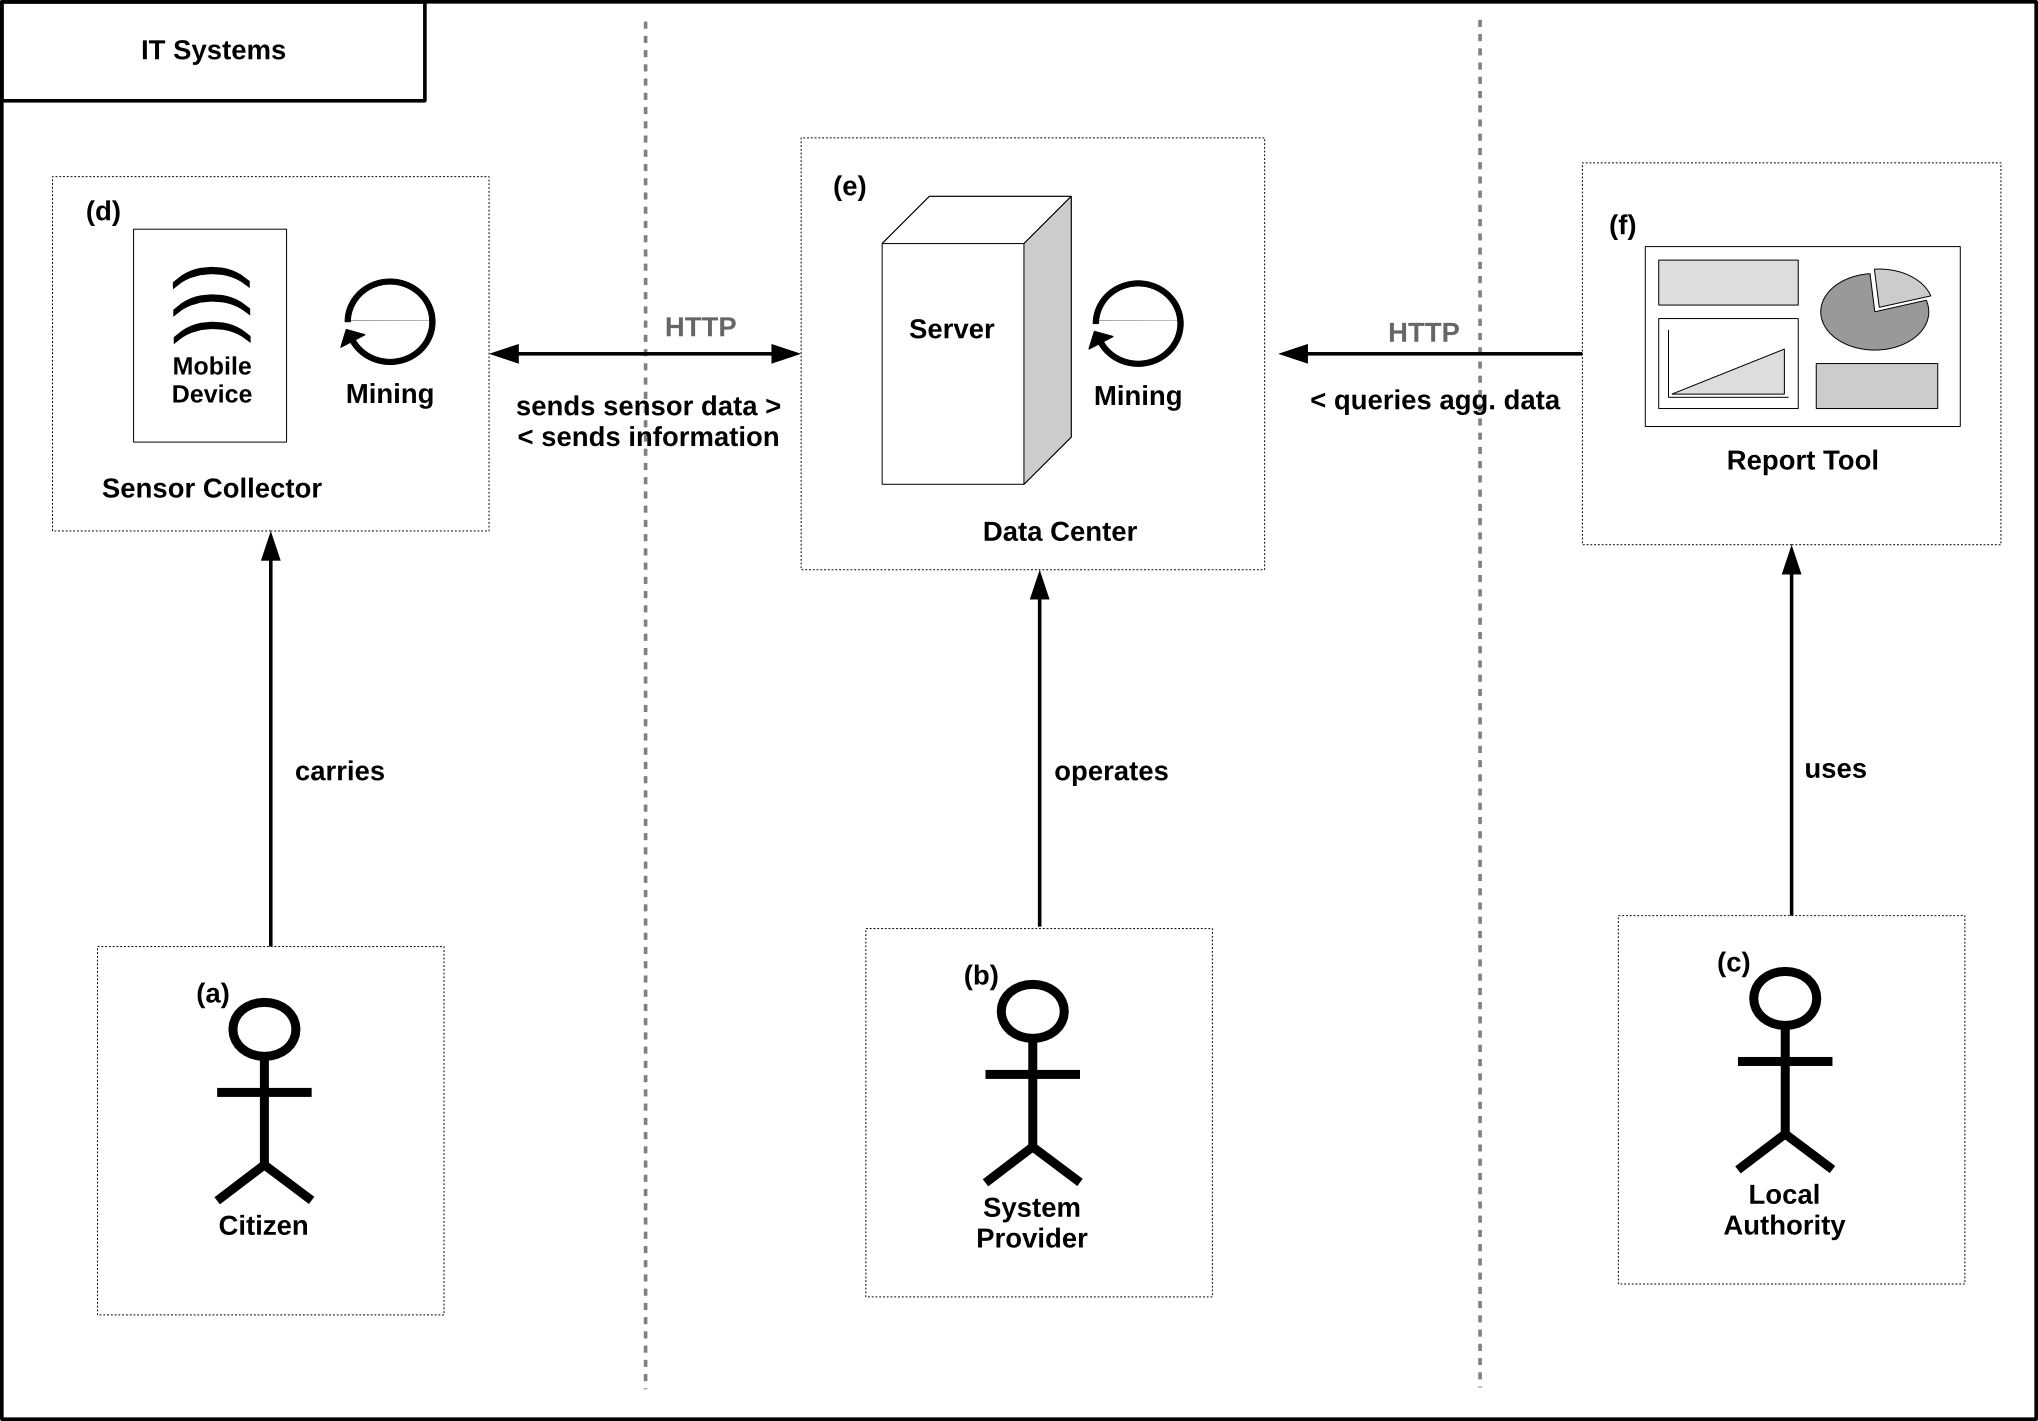
\includegraphics[width=0.7\textwidth]{diagrams/png/it-systems.png}

\begin{flushleft}
\scriptsize
\textbf{Legend:}
\begin{itemize}
\itemsep1pt\parskip0pt\parsep0pt

\item
\textbf{(a) Citizen:} 
User of the L+G client application whose privacy is at stake.

\item
\textbf{(b) Service Provider:} Provides technical infrastructure.

\item
\textbf{(c) Local Authority:} Provider of the L+G system.

\item
\textbf{(d) Mobile Device:}
Runs the L+G client application, produces and stores data sensitive to the users privacy.

\item
\textbf{(e) Data Center:} Runs the L+G services, processes and stores user data.

\item
\textbf{(f) Report Tool:} Interface to aggregated user data.

\end{itemize}
\end{flushleft}

\caption{IT Systems}
\label{figure:IT Systems}
\end{figure}

A \emph{citizen} (a) carries a mobile device running the \emph{sensor collector} application (d).
The sensor collector application is able to collect various kinds of sensor data (accelerometer, GPS, GSM, ...) and can sent the raw data back to the \emph{data center} (c).
The sensor collector can also be able to perform certain data mining operations.

Examples of such data mining operations include human activity recognition,the detection of service lines, detection of characters and faces from images.

In the Live+Gov Project mobile devices are used in particular for the following activities:
\begin{enumerate}
\item collection of GPS samples,
\item mining of Human activities (HAR) based on accelerometer samples,
\item collection of reports consisting of an image, free text and selected categories.
\end{enumerate}

The \emph{data center} stores and processes sensor data collected with the sensor collector application. It can also take into account data obtained from third parties, like the current positions of trains.
The data center can sent mining end products (traffic jam reports, bus schedule) back to the mobile device of the citizen.

In the Live+Gov Project data centers, in particular, perform the following activities:
\begin{enumerate}
\item storage of login credentials, name, and email address for each citizen,
\item storage of collected GPS samples (user id, timestamp, GPS location),
\item storage of HAR results (user id, timestamp, HAR result),
\item detection of service lines based received GPS samples (SLD),
\item storage of SLD results (userid, timestamp, SLD result),
\item sent back SLD results to mobile device,
\item storage of received reports (user id, timestamp, report),
\item detection of inherent patterns of the received reports.
\end{enumerate}

The \emph{System Provider} (b) provides and operates technical infrastructure like the Data Center and the \emph{Reporting Tool} (f).
The Reporting Tool queries the Data Center for aggregated data to visualize in form of charts and other means suitable to help understanding of monitored citizens.

\textit{Local Authorities} (c) use the reporting tool to get information in order to understand citizen movement and improve public services.
In such systems, the most valuable information for local authorities is not the raw sensor data, but aggregated views on the mining end products.

In the Live+Gov Project the reporting tools allows, in particular the following queries:
\begin{enumerate}
\item show aggregate information about which routes citizens take starting from a given location,
\item show the average waiting time of a citizen for each bus stop,
\item show routes where citizens where running to catch a bus,
\item show locations of all reports in a given time window,
\item visualize detected patterns in the report data,
\item view individual reports.
\end{enumerate}
\end{LGContent}


%============================================================

\section{Definition of Privacy}
\label{sec:privacydef}

%\TODO{MM:\\
%- Shorten\\
%- DONE - Remove Implicit Type Violations\\
%- Update figure\\
%- RG: Discuss alternative definitions of privacy\\
%}

\noindent
Defining privacy is a challenge which seems impossible. This is well put to words by Serge Gutwirth, who notes:
\begin{quote}
The notion of privacy remains out of the grasp of every academic chasing it. Even when it is cornered by such additional modifiers as `our' privacy, it still finds a way to remain elusive. \cite{Gutwirth}
\end{quote}
In this section we introduce the concept of privacy as control over information.
We specify types of information we have to deal with in the context of privacy.
And finally we outline the impact mobile sensors can have on one's privacy.

\subsection{Privacy as Control over Information}
%We may need to remove the following paragraph depinding on RG's alternative definition of privacy
%Many definitions seem to focus on the vulnerabilities of privacy.
%Thus a great amount of work is invested in finding threats to prohibit instead of describing why privacy is so valuable to us.
%This way around one could derive measures to ensure and secure its value. \cite{7ToP}

%One particular scholar, who did not follow this way of thinking is Charles Fried.
One possible definition of privacy is given by Charles Fried in his work \textit{An Anatomy of Values}\cite{CFried:Privacy}.
He questioned, why we are intuitively sensitive to privacy violations.
But he did not assert privacy as an intrinsic value by itself, he rather stated:
\begin{quote}
\textbf{Privacy is} not simply an absence of information about us in the minds of others;
rather it is \textbf{the control we have over information about ourselves}. \cite{CFried:Privacy}
\end{quote}
According to Fried privacy is our ability to create and modulate the relationships to other humans.
Which makes us intuitively sensitive for its violation, because this affects what defines our identity.
Also, the ability to build and maintain relationships is essential to society.
This is what makes privacy valuable and deserving of protection. 
\cite{sep-privacy}\cite{CFried:Privacy}

\subsubsection{Relationship Creation.}

% Privacy + Trust ~> Relationship
% ===============================
% - A shares intimate information with B
% - A trusts B not to reveal that information by not constantly monitoring B, i.e. respecting B's privacy
% - B has now the possibility to share intimate information with A

We share information of great intimacy only with persons we deem trustworthy. 
Moreover, we trust those persons to not reveal information about us to others by not constantly monitoring them, i.e. respecting their privacy.
Trust needs the possibility of unknown failure.
If we would constantly monitor our partners, they cannot fail unnoticed nor can they willingly share intimate information with us.
By trusting them, we create the possibility for them to share intimate information with us.
\cite{CFried:Privacy}

\subsubsection{Relationship Modulation.}
Fried argues, depending on the person we are interacting with, we are changing the degree of intimacy we share.
If we are to share private information with others, we are most likely aware that this action is privacy related.
In that case we are able to selectively disclose information along the two dimensions of quantity and quality.
\cite{CFried:Privacy}

\subsubsection{Alternative Definitions.}
Using Fried's anatomy of privacy for this analysis is suitable because of two points.
Despite the fact his text was published in 1970, he already included technologies to its viewpoint that did not only monitor location, but also record biometric data \cite{CFried:Privacy}. 
Secondly, the concept of control over information does not enforce data minimization.
Fried's definition complies with what we call \textit{self data protection}, where persons communicate their data self-determined.
This is the opposite of \textit{system data protection}, where the collection of certain data is prohibited. 

\TODO{RG: Discuss alternative definitions of privacy}

%=======================================================================================



\begin{LGContent-Hidden}
Defining privacy is a challenge which seems impossible. This is well put to words by Serge Gutwirth, who notes:

\begin{quote}
The notion of privacy remains out of the grasp of every academic chasing it. Even when it is cornered by such additional modifiers as `our' privacy, it still finds a way to remain elusive. \cite{Gutwirth}
\end{quote}

%Many researchers seem to only ``focus on the ways in which privacy can be infringed'' \cite{7ToP}.
%Thus they try to create taxonomies of \emph{privacy harms} instead of taxonomies of \emph{privacy types}.
%Those two differ in the respect that the former focuses on threats to prohibit whereas the latter focuses on values to protect.
%So one should rather evaluate what aspects are precious about privacy and develop measures to ensure their security than only forbid single actions against it \cite{7ToP}.

Many researchers seem to only ``focus on the ways in which privacy can be infringed'' \cite{7ToP}.
Thus they invest a great amount of work in defining threats to prohibit instead of describing why privacy is so valuable to us.
This way around one could derive measures to ensure and secure its value \cite{7ToP}.
One particular scholar who does this in the context of digital monitoring is Charles Fried.
He questioned, why we are intuitively sensitive to violations of privacy.
But he did not assert privacy as an intrinsic value by itself, he rather sated:

\begin{quote}
Privacy is not simply an absence of information about us in the minds of others;
rather it is \textbf{the control we have over information about ourselves}. \cite{CFried:Privacy}
\end{quote}

According to Fried privacy is a \textit{rational context}.
Which means that one is aware of such context's existence during a rational action.
If we are to share private information with others, we are most likely aware that this action is privacy related.
In that case we are able to selectively disclose information along the two dimensions of quantity and quality.
This leads Fried to his thesis, that privacy is one's ability to create and modulate his or hers social relationships, namely: friendship, love and trust. \cite{CFried:Privacy}

Depending on the conversation partner, we change the degree of intimate information we share if it is a total stranger, colleague, close friend or lover.
With close friends or lovers we share information of great intimacy we do not share with anyone else.
Moreover, we trust those persons to not reveal information about us to others by respecting their privacy.
Trust needs the possibility of unknown failure.
If we would constantly monitor our partners, they cannot fail unnoticed nor can they willingly share that information with us.
Thus they could not trust us anymore. \cite{CFried:Privacy}

So privacy or the its possibility, according to Fried, is the foundation of our core relations: friendship, love and trust.
And thus it is valuable, because those relations are essential to human society \cite{CFried:Privacy}.
Using his anatomy of privacy as foundation of our analysis is suitable because of two points.
At first, Fried's study on the understanding of privacy provided a great contribution to the research on the same term in philosophy \cite{sep-privacy} and computer science \cite{SociotechnicalArchitectureForOnlinePrivacy}.
Secondly, despite the fact his text was published in 1970, he already included technologies to its viewpoint that did not only monitor location, but also record biometric data.
\end{LGContent-Hidden}

\subsection{The Seven Types of Privacy}
\label{sec:privacytypes}

In Fried's definition of privacy as control over information, the specification of what constitues such information remains open.
There is a vast amount of information that relates to a person and we need to get a better understanding in order to perform a thorough analysis.
To this end we use the the categorization by Friedewald, Finn and Wright \cite{7ToP} called the \textit{Seven Types of Privacy}.
The seven types of privacy are an extension to the four types of privacy by Roger Clarke \cite{RClarke:4ToP}, which are:
\textit{Privacy of the Person},
\textit{Privacy of Personal Behaviour},
\textit{Privacy of Personal Communication},
\textit{Privacy of Personal Data}.
It is important to note, that these categories do not form a taxonomy, since the categories are not mutually exclusive.
For instance a written email is considered personal communication as well as personal data stored on a computer.

Moreover, Friedewald et al. argue that Clarke's types are outdated and no longer adequate in order to describe the privacy aspect of our modern, technology driven, world.
In order to address this shortcoming they extend the former four to the now introduced seven types privacy as follows:

\begin{enumerate}

\item \textbf{Privacy of the Person}
This privacy type is generally concerned with one could best understand as biometric privacy.
Friedewald et al. paraphrase it as \emph{``\om the right to keep body functions and body characteristics \om private''}.
This includes but is not limited to measures like weight, height or shoulder width;
biometric identifiers like fingerprints and DNA sequences;
or medical conditions such as limping or having a cold.


\item \textbf{Privacy of Behaviour and Action}
This privacy type is concerned with one's activities in public as well as in private spaces.
It includes but is not limited to religious practices, political activities and sexual preferences or habits.


\item \textbf{Privacy of Communication}
This privacy type is concerned with one's communication in a broad sense.
It includes written correspondence, but also conversations conducted either vis-a-vis or via electronic devices.
Friedewald et al. put it as the right to free discussion without unknown interception by third parties.


\item \textbf{Privacy of Data and Image}
This privacy type is concerned with the secrecy of personal data, especially its automatic disclosure to other individuals and organizations.
It includes data such as paychecks, insurance information or records of public administration.
However, it also refers to pictures taken without consent and digital identifiers like IP addresses or social security numbers.


\item \textbf{Privacy of Thoughts and Feelings}
This privacy type is the counterpart to Privacy of the Person like body and mind are counterparts of one another.
Comparable to the Privacy of Data and Image, Friedewald et al. state that one's thoughts and feelings must not be automatically revealed to others.
This could simply happen by the disclosure of one's diary or by technologies which allow emotion detection through biometric means.
One's body temperature or iris reflexes might infer stress or excitation.


\item \textbf{Privacy of Location and Space}
This privacy type is concerned with one's movements in public spaces and the protection of private spaces.
Friedewald et al. qualify the first dimension as one's right to move without being identified, tracked or monitored.
The second dimension is qualified as one's general right to solitude, especially the right to the inviolability of the home.


\item \textbf{Privacy of Association}
This privacy type is also put as group privacy.
Friedewald et al. state that one must have the possibility with whomever without being recorded.
Associations like friends or organizations such as political parties must not automatically be recorded because one associates with them, and vice-versa.
\end{enumerate}

\begin{LGContent-Hidden}
In Fried's definition of privacy as control over "information about onself'', the specification of what constitues such information remains open.
There is a vast amount of information that relates to a person and we need to get a better understanding in order to perform a thorough analysis.
To this end we use the the categorization by Friedewald, Finn and Wright \cite{7ToP} called the \textit{Seven Types of Privacy}.
The seven types of privacy are an extension to the four types of privacy by Roger Clarke \cite{RClarke:4ToP}, which are:
\textit{Privacy of the Person},
\textit{Privacy of Personal Behaviour},
\textit{Privacy of Personal Communication},
\textit{Privacy of Personal Data}.
It is important to note, that this categories do not form no taxonomy, since the categories are not mutually exclusive.
For instance a written email is considered personal communication as well as personal data stored on a computer.

Moreover, Friedewald et al. argue that Clarke's taxonomy is outdated and no longer adequate in order to describe the privacy aspect of our modern, technology driven, world.
In order to address this shortcoming they extend the former four to the now introduced seven types privacy as follows:

\begin{enumerate}

\item \textbf{Privacy of the Person}
This privacy type is generally concerned with one could best understand as biometric privacy.
Friedewald et al. paraphrase it as \emph{``\om the right to keep body functions and body characteristics \om private''}.
This includes but is not limited to measures like weight, height or shoulder width;
biometric identifiers like fingerprints and DNA sequences;
or medical conditions such as limping or having a cold.


\item \textbf{Privacy of Behaviour and Action}
This privacy type is concerned with one's activities in public as well as in private spaces.
It includes but is not limited to religious practices, political activities and sexual preferences or habits.


\item \textbf{Privacy of Communication}
This privacy type is concerned with one's communication in a broad sense.
It includes written correspondence, but also conversations conducted either vis-a-vis or via electronic devices.
Friedewald et al. put it as the right to free discussion without unknown interception by third parties.


\item \textbf{Privacy of Data and Image}
This privacy type is concerned with the secrecy of personal data, especially its automatic disclosure to other individuals and organizations.
It includes data such as paychecks, insurance information or records of public administration.
However, it also refers to pictures taken without consent and digital identifiers like IP addresses or social security numbers.


\item \textbf{Privacy of Thoughts and Feelings}
This privacy type is the counterpart to Privacy of the Person like body and mind are counterparts of one another.
Comparable to the Privacy of Data and Image, Friedewald et al. state that one's thoughts and feelings must not be automatically revealed to others.
This could simply happen by the disclosure of one's diary or by technologies which allow emotion detection through biometric means.
One's body temperature or iris reflexes might infer stress or excitation.


\item \textbf{Privacy of Location and Space}
This privacy type is concerned with one's movements in public spaces and the protection of private spaces.
Friedewald et al. qualify the first dimension as one's right to move without being identified, tracked or monitored.
The second dimension is qualified as one's general right to solitude, especially the right to the inviolability of the home.


\item \textbf{Privacy of Association}
This privacy type is also put as group privacy.
Friedewald et al. state that one must have the possibility with whomever without being recorded.
Associations like friends or organizations such as political parties must not automatically be recorded because one associates with them, and vice-versa.
\end{enumerate}

\end{LGContent-Hidden}


\subsection{Sensor Data Privacy Impact}
\label{sec:SensorPrivacyImpact}

Modern mobile devices have a broad collection of sensors.
Disclosure or processing of sensor data can impact one's privacy.
In this section we identify groups of sensors and their potential impact on a certain type of privacy.
Figure \ref{figure:Sensor Data Privacy Impact Matrix} qualifies that impact on a simple scale.
Privacy of Data and Image is trivially threatened because here sensor data is individual data, a priori.
Indirect impact is caused by combining sensor data with additional knowledge.
For instance, comparing a contemporary map with locational data can imply behaviour if the position matches a church.

\begin{figure}
\newcommand{\tcell}[1]{\parbox[c][2cm]{4cm}{\vspace{3mm}#1\vspace{3mm}}}
\newcommand{\thead}[1]{\tcell{\Large\centering\textbf{#1}}}
\newcommand{\tbody}[1]{\tcell{\Large\centering #1}}
\centering
\resizebox{\textwidth}{!}{
\begin{tabular}{|c||c|c|c|c|c|c|c|}
\hline
& \thead{Pricacy of the Person}
& \thead{Pricacy of Behaviour and Action}
& \thead{Pricacy of Communication}
& \thead{Pricacy of Data and Image}
& \thead{Pricacy of Thoughts and Feelings}
& \thead{Pricacy of Location and Space}
& \thead{Pricacy of Association}
\\\hline\hline
\thead{GPS Sensor}
& \tbody{0.5} % Pricacy of the Person
& \tbody{0.5} % Pricacy of Behaviour and Action
& \tbody{0} % Pricacy of Communication
& \tbody{1} % Pricacy of Data and Image
& \tbody{0} % Pricacy of Thoughts and Feelings
& \tbody{1} % Pricacy of Location and Space
& \tbody{0.5} % Pricacy of Association
\\\hline
\thead{Motion Sensors}
& \tbody{1} % Pricacy of the Person
& \tbody{0.5} % Pricacy of Behaviour and Action
& \tbody{0} % Pricacy of Communication
& \tbody{1} % Pricacy of Data and Image
& \tbody{0} % Pricacy of Thoughts and Feelings
& \tbody{0} % Pricacy of Location and Space
& \tbody{0} % Pricacy of Association
\\\hline
\thead{Networking Sensors}
& \tbody{0.5} % Pricacy of the Person
& \tbody{0.5} % Pricacy of Behaviour and Action
& \tbody{0} % Pricacy of Communication
& \tbody{1} % Pricacy of Data and Image
& \tbody{0} % Pricacy of Thoughts and Feelings
& \tbody{1} % Pricacy of Location and Space
& \tbody{1} % Pricacy of Association
\\\hline
%\thead{HAR}
%& \tbody{-} % Pricacy of the Person
%& \tbody{-} % Pricacy of Behaviour and Action
%& \tbody{-} % Pricacy of Communication
%& \tbody{-} % Pricacy of Data and Image
%& \tbody{-} % Pricacy of Thoughts and Feelings
%& \tbody{-} % Pricacy of Location and Space
%& \tbody{-} % Pricacy of Association
%\\\hline
%\thead{SLD}
%& \tbody{-} % Pricacy of the Person
%& \tbody{-} % Pricacy of Behaviour and Action
%& \tbody{-} % Pricacy of Communication
%& \tbody{-} % Pricacy of Data and Image
%& \tbody{-} % Pricacy of Thoughts and Feelings
%& \tbody{-} % Pricacy of Location and Space
%& \tbody{-} % Pricacy of Association
%\\\hline
\end{tabular}
}
\newline
\newline
{\scriptsize 
0: No Impact,
0.5: Indirect Impact,
1: Direct Impact}
\caption{Sensor Data Privacy Impact Matrix}
\label{figure:Sensor Data Privacy Impact Matrix}
\end{figure}

\subsubsection{GPS Sensor.}
The GPS sensor gives the current longitude and latitude, the current global position of the mobile device and its carrier, although there is some artificial inaccuracy within civil use. Therefore, the collection of GPS data violates directly the citizens privacy of Location and Space.

%By inference we also get implicit violations of the Privacy of the Person, Privacy of Behavior and Action and Privacy of Association.

\subsubsection{Motion Sensors.}
Accelerometer, Rotation Vector, Gyroscope and Magnetic field sensor measure the physical movement of the mobile device on all three axes.
If the mobile device is carried ``normally'' its safe to say that those sensors also measure the moments of its carrier.
So his privacy is infringed regarding biometric behaviour, i.e. the Privacy of the Person.

%By inference we also get implicit violations of the Privacy of Behavior and Action.

\subsubsection{Network Sensors.}
The GSM and WLAN sensors reveal the position of the mobile device and its carrier, when used in connection with external databases.
The both sensors give the exact cell or network, the mobile device has registered with at the current moment.
Frequent connection to one particular network also reveals association, e.g. university networks.

The Bluetooth sensors record lists of the bluetooth clients in the direct neighbourhood.
Since those clients are usually moving, inference of the position is usually not possible.
Instead, bluetooth clients carried by a third person may infringe the Privacy of Association.

%A similar argumentat applies to WLAN snsors. 
%If one frequently connects with an organizational wireless network, e.g.~an university network, an association can be deduced (student or staff).

%\subsubsection{Human Activity Recognition.}
%The detection and collection of human activities like walking, standing and running, can interfer with the Privacy of the Person, e.g.~since these movement patterns can be indicators for a person's health. Also, trivially, Privacy of Data and Image is violated.
%
%\subsubsection{Service Line Detection.}
%The detection and collection of the service line the user currently uses in the public transportation system allows inference of the location of the user, at least when entering and leaving those service lines at e.g.~bus stops.
%Implicit privacy violations apply accordingly.


\begin{LGContent-Hidden}

%input{./figures/LG-Implicit-Sensor-Privacy-Matrix}

%TODO: Reformulate the section.
% - Too much overlap with preceeding sections.
% - Structure should be per Sensor Type
% - Add HAR and SLD!

In this section we analyze the impact of the disclosure sensor data and certain processing results to the citizens privacy.
This analyisis builds upon the preceeding analyis, but is more focused on the concrete type of data vailable.
For example, the disclosure of Service Line Detection results, does violate the Privacy of Location and Space but not the Privacy of Association that is violated by general GPS tracking.

\textbf{GPS Data}.
The GPS sensor gives the current longitude and latitude, the current global position of the mobile device and its carrier, although there is some artificial inaccuracy within civil use. Threefore, the collection of GPS data violates directly the citizens privacy of Location and Space, and the privacy of Data an Image.

By inference we also get implicit violations of the Privacy of the Person, Privacy of Behavior and Action and Privacy of Association.

\textbf{Motion Sensors.}
Accelerometer, Rotation Vector, Gyroscope and Magnetic field sensor measure the physical movement of the mobile device on all three axes.
If the mobile device is carried ``normally'' its safe to say that those sensors also measure the moments of its carrier.
So his privacy is infringed regarding biometric behaviour, as it is captured automatically
Privacy of Data and Image is trivially threatened because here sensor data is individual data, a priori.

By inference we also get implicit violations of the Privacy of Behavior and Action.

\textbf{Network Sensors.}
The GSM and WLAN sensors reveal the position of the mobile device and its carrier, when used in connection with external databases.
The GSM sensor gives the exact cell, the mobile device has registered with at the current moment.

The Bluetooth sensors record lists of the bluetooth clients in the direct neighbourhood.
Since those clients are usually moving, inference of the position is usually not possible.
Instead, bluetooth clients carried by a third person may infringe the Privacy of Association.

A similar argumentat applies to WLAN snsors. If one frequently connects with an organizational wireless network, e.g.~an university network, an association can be deduced (student or staff).

\textbf{Human Activity Recognition.}
The detection and collection of human activities like walking, standing and running, can interfer with the Privacy of the Person, e.g.~since these movement patterns can be indicators for a person's health. Also, trivially, Privacy of Data and Image is violated.

\textbf{Service Line Detection.}
The detection and collection of the service line the user currently uses in the public transportation system allows inference of the location of the user, at least when entering and leaving those service lines at e.g.~bus stops.
Implicit privacy violations apply accordingly.

\end{LGContent-Hidden}

%============================================================








\section{Privacy Analysis}


The goal of this chapter is to analyze and identify the threads to
personal privacy that are posed by collecting, storing and processing
sensor data from mobile phones.  We derive concrete privacy protection
measures that address the main risks involved with handling such data.


In section \ref{subsec:world-analysis} and \ref{subsec:pot-analysis} we apply the first two steps of the Reference Model for IT Security Analysis as described in \cite{Grimm:ItSecRefModel}.  It supersedes earlier efforts by
e.g. \cite{Avizienis}.  The reference model consists of a \emph{model}
and a \emph{procedure}: The model aims to organize common security terminology in a reasonable and practical way. The procedure describes a method to analysis the IT system based on that model. In these sections we give a brief overview over the reference model by applying it to our scenario.


In section \ref{subsec:priv-rec} we provide specific privacy recommendations and requirements as a result of the previous analysis that the system must comply with.

\subsection{Step 1. World Analysis}

\label{subsec:world-analysis}

The first step is the \emph{world view} where all components are described in their current state. It consists of the following components:
\begin{itemize}
	
	\item \textbf{Assets.} 
	Things of value to one or more stakeholders.
	
	\item \textbf{IT-Systems.}
	The relevant IT-Systems under study. Already described in Section \ref{subsubsection:it-systems}.
		
	\item \textbf{Actors.}
	All identifiable stakeholders of the system under study.
	
	\item \textbf{Conflicts of Interests.}
	Different actors have different interests which can be in conflict which each other.
	
	\item \textbf{Vulnerabilities.}
	All identifiable weaknesses in the IT-System e.g. a weak passwords.
	
	\item \textbf{Interactions.}
	This point captures all possible interactions between assets, IT-Systems, humans, and vulnerabilites as partly described in Section \ref{subsubsection:it-systems} and will be further analyzed in \ref{subsec:pot-analysis}.
	
\end{itemize}


\subsubsection{Assets}

In this scenario we focus our attention to only one asset: The privacy of the citizen.
Our definition of privacy is described in detail in Section \ref{sec:privacydef} and introduced in Section \ref{sec:privacytypes} the seven different types of privacy.


\subsubsection{Actors}
\label{subsubsection:humans}

This section describes the human actors previously introduced within the IT system architecture (\ref{subsubsection:it-systems}).
Also the additional actor \textit{External} is introduced as a person with no special access rights. Although the text is only a short description, a list of the most important interests is provided for each actor.

\textbf{Citizen.}
Citizens are persons who use the mobile device as users of the provided software.
Their main motivation for using the software is to gain a higher level of convenience in their daily activities. For example they may have access to real time bus schedules or reports about traffic jams, that help them to avoid long waiting times. Also they generally benefit from improvements of public infrastructure by local authorities, which is triggered by issue reports.

By using the application, citizens are sharing personal information like name and address, as well as data gathered from mobile sensor with the service provider. This data can be exploited in ways that are harmful to the citizen (cf. \cite{GuardienMassSurveillance}).

Citizens are interested in: physical wellbeing and health, financial profit, convenience, legitimate use of personal data, non-disclosure of personal data to peers of the citizen, and not being monitored.

\textbf{External.}
Externals are persons who do not have privileged access to the IT systems, and are willing to break laws, security constrains and norms in order to promote their interests. 

A common interest of an external is financial profit. For example they want to obtain access to critical systems to steal sensitive data or to get the system under their control. Stolen data could simply be sold as is or used for illegitimate purposes, e.g. spam or phishing attacks - or excessive data mining.

In short, externals could be interested in: increase power over citizen, financial profit, political activism, and their social standing.

\textbf{System Provider.}
System Providers operate the technical infrastructure (hardware and software) of the IT System.
They are private companies and legal persons in their own right, but also employ a number of people with diverging interests including administrators, programmer/developer, and a support manager.

As companies, they are interested in gaining financial profit. The financial success of system providers depends on the task complexity of the maintained infrastructure. The complexity of a task has to be in reasonable bounds, so that system providers can complete it within time, with a satisfying quality.

System Providers are interested in: financial profit, manageable complexity, professional excellence, and good working conditions.

\textbf{Local Authority.}
Local authorities are public offices (ministry, agency, department, ...) or other external public entities which act as direct customers of service providers.
They purchase a system specialized for their needs.
For example a department for urban mobility, orders a system to better understand usage patterns and make improvement to the urban traffic flow. Such systems are investments, and so naturally local authorities are interested in a profitable return, like increased ticket sales.

Local authorities are interested in: financial profit, political reputation, business intelligence, and good working conditions.


\subsubsection{Conflicts of Interests}
\label{subsubsection:Conflicts of Interests}
Different actors have different interests which can be in conflict each other. This section outlines the Conflicts of Interests between the actors of the proposed IT system architecture.

The individual interests of all actors is already described in the previous section and are not elaborated any further.
The emphasis here is put on prominent existing conflicts, because they provide a foundation for vulnerabilities and subsequent threats.


\textbf{System Complexity vs Privacy.}
System Providers offer a service to Local Authorities, so that Local Authorities can improve their public services. This task in it self has a high technical complexity and operates on privacy sensitive data provided by monitored Citizens.

\textbf{Business Intelligence vs Privacy.}
Local authorities order a monitoring and mining system from system providers as much as possible, which allows them to produce business intelligence for public services. They are interested in the successful usage of their data, although the interest of citizens lies in maintaining control over their data and protecting their rights to privacy.

\textbf{Power of External vs. Privacy.}
Externals which are in a social relation to the citizen can have an interest in obtaining further information in order to gain power. In the most simplistic example this could be a man wanting monitor the activities of his spouse.


\textbf{Financial Profit of External vs Privacy.}
Externals can gain financial profit from stealing privacy sensitive data.
For example by selling raw contact information to advertisers or by selling mined data to insurance companies, or intermediaries like scoring companies. In such cases, citizens lose complete control over their data.


\textbf{Financial Profit of External vs Reputation of System Providers.}
Externals have various business models as optional foundation for attacks on System Providers.
For instance, they can try to invade the infrastructure for e-espionage reasons, to get control over servers to create a bot network or to steal user data. A successful attack proves the technical competence of system providers wrong and subsequently harms their professional reputation.


\textbf{Political Activism vs Reputation of Local Authority.}
Besides monetary reasons, externals can be motivated by political reasons to attack the monitoring and mining system.
Externals can break the system to make a political statement of their own,
or they can steal user data to prove the system insecure.
Both would harm the reputation of local authorities, who endangered the privacy of the citizens.


\subsubsection{Vulnerabilities}
\label{subsubsection:Vulnerabilities}
This section outlines the vulnerabilities (Figure \ref{figure:Live+Gov Vulnerabilities}) of the proposed monitoring and mining system.
Note that vulnerabilities are not necessarily of technical nature.
The weaknesses of IT systems are often created due to misuse or misconfiguration of the various components by one or more actors.

%input{./figures/LG-Vulnerabilities}
\begin{figure}
\centering
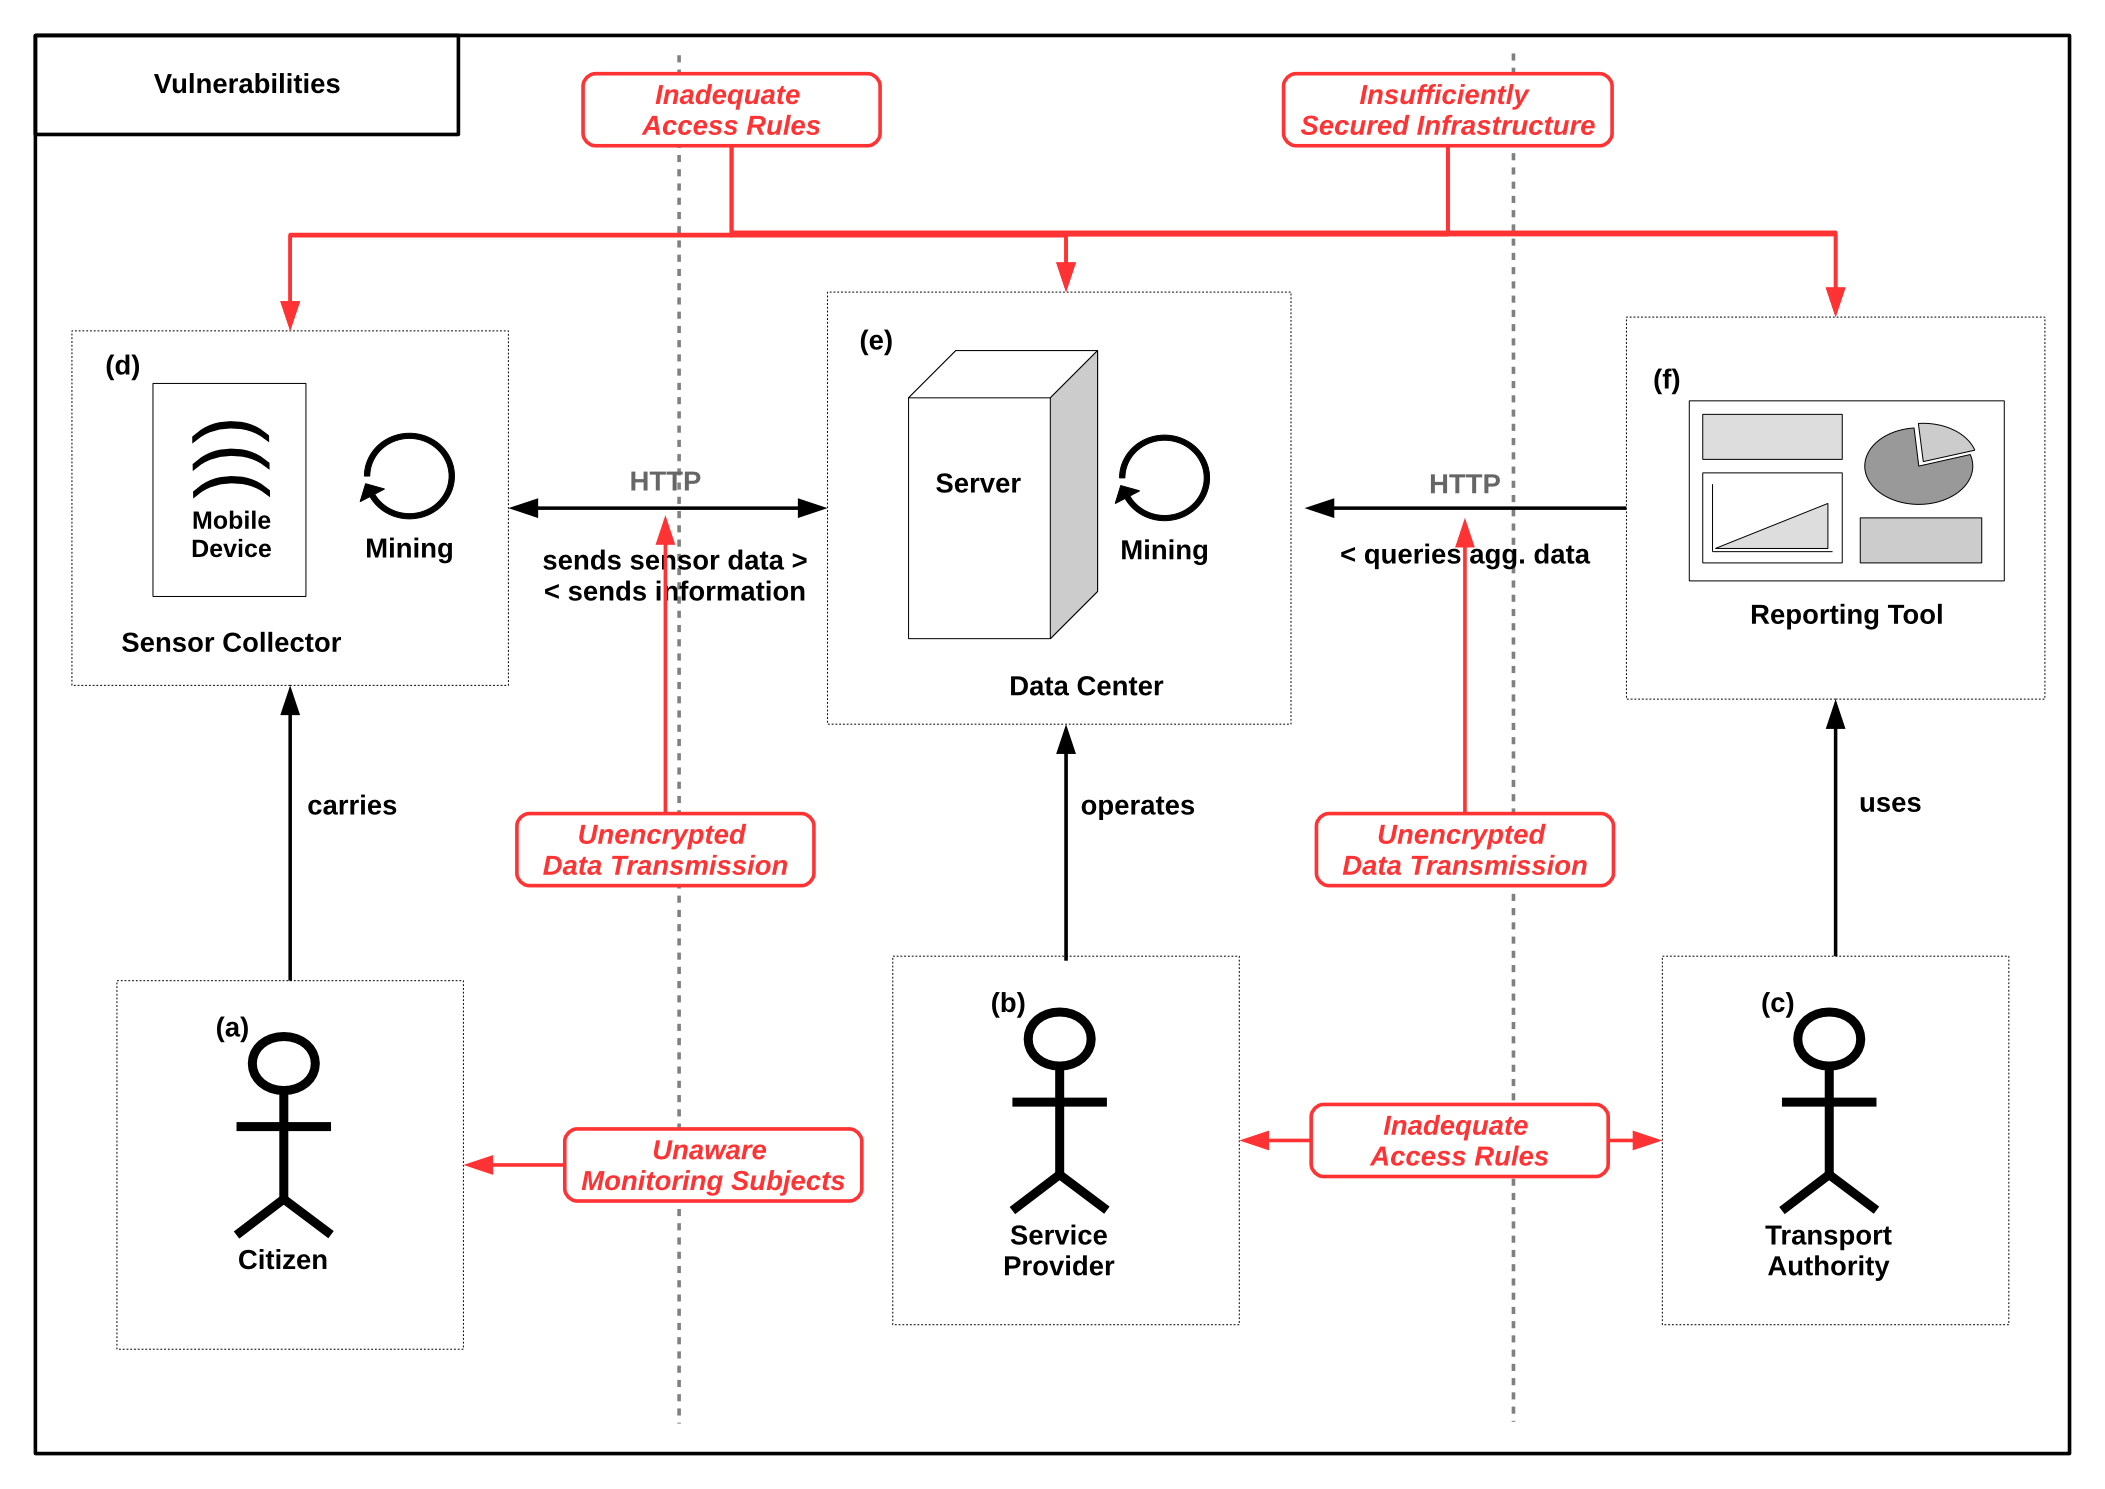
\includegraphics[width=0.8\textwidth]{diagrams/png/vulnerabilities.png}

\caption{Overview of vulnerabilities of the Live+Gov System; legend see \ref{figure:IT Systems} }
\label{figure:Live+Gov Vulnerabilities}
\end{figure}

\textbf{Insecure Infrastructure.}
The proposed monitoring system consists of many hardware and software components, each with its own concrete weaknesses. For instance, operating systems can be outdated or not subject to frequent updates or virus scans.

\textbf{Insecure Data Transmission.}
The proposed monitoring and mining system uses HTTP to exchange data between the Sensor Collector, the Data Center and the Report Tool.
Data can be intercept and read all sensitive information, which is send between the components e.g. passwords, raw sensor data and data mining results.

\textbf{Unhappy Employees.}
An Employee that is frustrated with his situation for a long time
period constitutes a security vulnerability. On the one hand he might
want to harm his employer directly, on the other he is increasingly
susceptible for social engineering.

\textbf{Inadequate Access Rules.}
The proposed IT system infrastructure has various accesses to privacy sensitive data.
System Provider staff has access to Data Center hardware and software like databases, web-servers and other inspection tools. Local Authority staff has access to the Report Tool. This all enables staff members to have potential access to privacy sensitive information.


\textbf{Unaware Monitoring Subjects.}
We define privacy as one's ability to control information about
oneself.  In order to do that, monitored subjects need to know, that
they are monitored, who monitors them, what information is recorded
and for what purposes.  Subjects who are not aware of these things
cannot effectively preserve control and thus lose their privacy. 

\subsection{Step 2. Potential Analysis}
\label{subsec:pot-analysis}

The \emph{Potential Analysis} (or \emph{Potential View}) displays the intended and unintended interactions of the components in the world view.
The intended interactions support the underlying business objectives.
Unintended interactions lead to threats. The potential view consists of the following components:

\begin{itemize}

	\item \textbf{Business Objectives.}
	Interaction of IT-system and actors that realize a business goals of the system owner were already described in Section \ref{subsubsection:it-systems} and \ref{subsec:world-analysis}.

	\item \textbf{Threats.}
	A threat is a potential interaction that destroys or harms assets of the system.
	Concrete realizations of threats can be \emph{attacks} or \emph{accidents}.
	Attacks are executed by an actor in response to a conflict of interest.
	Accidents are harmful interactions that are not willfully caused by an actor.
	
	\item \textbf{Chances/Risk.}
	Evaluation of chances and risks associated to the business objectives and threats. The risk associated to a threat is its expected loss.

	\item \textbf{Security Requirements.}
	Interactions (e.g. threats) that shall not occur within the system in order to achieve its business objectives.  We included these security requirements into our analysis in Section \ref{subsec:priv-rec}.
		
\end{itemize}


\subsubsection{Threat Specification}

A threat is a potential interaction of the components that targets an asset.
We restrict ourselves to the case of attacks, and the asset of privacy.
An attack is an interaction that is executed by an actor in response to a conflict of interest by exploiting a vulnerability of the system.
The alternative interaction of accidents are less relevant for us, since the violation of privacy always requires an actor that takes advantage of personal data.

We describe threats for the citizen privacy in the Live+Gov system.
This list can necessarily not be complete, but we make a best effort to cover the most relevant cases.


\textbf{T1. Insufficient Control Features.}
As soon as collected data of Citizens is stored on System Provider servers, all control over that data is lost. Although, control capabilities for Citizens add to the system complexity, which could motivate to omit those. Therefore interests of Citizens and System Providers are in conflict, namely it is the Citizen's \textit{Privacy vs. System Complexity} for System Providers. This is an abstract threat provoked by a general \textit{Missing Privacy Awareness} in the minds of all actors in the Live+Gov context.

\textbf{T2. Excessive Data Mining.}
The System Provider and/or the Local Authority secretly extract more private information from the collected data, than the Citizen agreed to.
But results of the mining process create no disadvantages for Citizens, because there is no disclosure to third parties.
This could be the case for a System Provider, who wants to test a new product and uses the pre-existing data collection.
Or for a Local Authority, who wants to analyze the data collection regarding fare evasion.
However, the Citizen has not agreed to such data processing nor could he, since it is conducted secretly.
This disables a Citizen to control his data adequately.
Thus there are two possible conflicts: \textit{Privacy vs. Financial Profit of Serivce Provider} and  \textit{Privacy vs. Buisness Intelligence of Local Authority}
The threat can be provoked by either lax data handling policies of both System Providers and Local Authorities, or a weak law enforcement of existing supervision.
But the main issue, which can lead to such threats, is again a general \textit{Missing Privacy Awareness}.

\textbf{T3. Data Theft}
An External infiltrates infrastructure in order to steal personal data and sell it on the black market. Also the External might be motivated politically and wants to harm the reputation of the System Provider or the Local Authority. Such a successful attack could harm the reputation of both System Provider and Local Authority. Thus this threat is defined by three conflicts: \textit{Privacy vs. Financial Profit}, \textit{Reputation of Service Provider vs. Political Activism} and \textit{Reputation of Local Authority vs. Political Activism}.
Also this threat describes the classical scenario, where attacks are provoked by \textit{Insecure Infrastructure} (SQL injection) and \textit{Insecure Communication} (Packet Capture).

\textbf{T4. Surveillance}
An External infiltrates infrastructure in order to obtain information
about the citizen and exploit it directly.  In this scenario the
external is supposed to have some direct relationship to the citizen
which motivates his interest to obtain personal information.  Examples
could be a public institution that wants to gain information about
planned activities of the citizens (e.g. Nixon's Watergate scandal or
the recent prosecution of Guardian journalists by GHCQ). 
In this threat the privacy interest of the citizen is in conflict with
the aspirations for power over the citizen by the externals.

\textbf{T5. Information Leak}

Like an external person the Data Theft Scenario an employee of the
service provider or the Local Authority has selfish interests to gain
money, make political statements or harm his employer.  In order to
pursue this interest he can steal personal data and sell it or release
it to the public.  The corresponding conflicts of interests are:
\textit{Privacy vs. Financial Profit} of the Employee, \textit{Reputation of Service
  Provider vs. Political Activism} of the Employee and \textit{Reputation of Local
  Authority vs. Political Activism} of the Employee.  The vulnerability constitutes of
the existence of \textit{Unhappy employees} itself and possibly \textit{lax access
rules} that enable the employee to obtain large amounts of data
unnoticed.

\textbf{T6. Social Engineering}
This scenario an external manipulates an employee of a Service
Provider or the Local Authority to leak information to the external
person.  It is thus combination of the Data Theft and Information Leak
scenario.
The conflicts of interest are \textit{Privacy vs. Financial Profit} of
the External, \textit{Reputation of Service Provider vs. Political
  Activism} of the external and \textit{Reputation of Local Authority
  vs. Political Activism} of the external.  The exploited
vulnerabilities are, again, the existence of \textit{Unhappy
  employees} and possibly \textit{lax access rules} that enable the
employee to obtain large amounts of data unnoticed.


\subsubsection{Threat Risk Evaluation}

In this section we will associate to every identified threat a corresponding risk. A risk is the expected loss that is associated to the threat.
Therefore, we have to quantify the likeliness of the threat to occure and the harm or loss done in this case.
The quantification of likeliness will be solely based on rough judgment of the authors.
The quantification of loss, will be made in a two step process.
For each threat listed in the previous section, we have analyzed the affected personal data of the citizen.
For each possible data type (e.g. GPS) we analyze the impact on the seven different types of privacy in Section \ref{sec:SensorPrivacyImpact}.
In combination we can quantify roughly the impact of each threat on the citizens privacy. Both evaluations are necessarily fraught with a high level of uncertainty.

For the quantification of the loss in case of a threat scenario we use the following rough calibration between 3 (high) and 0 (none). For the quantification of likeliness the following scale between 4 (always) and 0 (impossible) is used. The quantification of the risk, we add the values for loss and likeliness of the corresponding threats. Note, that loss and
likeliness scales have a logarithmic character, so that addition
of those scales corresponds to multiplication of the usual scales.

The likeliness, loss and the resulting risks assigned to the threats
are discussed in the following paragraphs and summarized in Figure
\ref{fig:risks}.

\textbf{T1. Insufficient Control Features.}  The occurrence of this
threat is dependent on the design on the system and given in our case,
since we do not give the citizen control over his data once it is
recorded. Therefore the Likeliness is evaluated as $4$ (Always).  The
associated, risk is $1$ Low on our scale, since no direct harm is done to
the citizen by exploiting the data.

Hence the resulting risk is calculated as $4+1 = 5$.

\textbf{T2. Excessive Data Mining.}
We assess the likeliness of excessive data mining to be $3$ High, since
these kind of analysis can be performed within the walls of the service
provider, without somebody else noticing, and the service provider himself
has an interest in this activity. The associated loss, on the other hand can be substantial (Medium $2$). 

Hence the resulting risk is calculated as $3+2 = 5$.

\textbf{T3. Data Theft.}
The likeliness of a targeted attack by a third party is dependent on
the popularity of the offered service and financial value of the
captured information. Moreover, the amount of manual work required to
infiltrate a custom build system is significantly higher that that of
compromising a standard software solution. In the scenario we assume a
moderate popularity in a single metropolitan area, with around 10.000
users and storage of data of only limited financial value (no
addresses, no payment information). Therefore the likeliness
assessment is $1-2$ (Low-Medium).

The harm of leaked information to a criminal party is $3$ High.
Hence the resulting risk is calculated as $4-5$.

\textbf{T4. Surveillance.}  In the surveillance scenario an party
related to the citizen, like a company where he is customer of, or a
government agency, seeks to obtain sensitive information from our
service.

The likeliness of such an intrusion is hard to asses, and depends
again on the popularity of the service. If a high popularity is
reached we have recently learned that spying by government agencies is
very likely to occur. The barrier for companies that do not operate
the infrastructure used to transmit the data a surveillance attack is
however very hard to perform. Therefore we assess the likeliness of
the threat with $1-2$ (Low-Medium).

The harm of leaked information to a related party is $3$ High.
Hence the resulting risk is calculated as $4-5$.

\textbf{T5/6. Information Leak and Social Engineering.}

In our scenario we assume that the culture and ethics inside the
service provider company and local authority are very high, so that
the information leak scenario has a likeliness of $1$ (Low).

The harm of such an information leaked is $3$ High, so that the
resulting risk is calculated as $4$.


\begin{figure}
\centering
\begin{tabular}{|l|l|l|l|l|}
\hline
\textbf{Threat}                   & \textbf{Likeliness} & \textbf{Loss} & \textbf{Risk} & \textbf{Recommendation}
\\\hline
T1. Insufficient Control Features & 4                   & 1             & 5             & R1, R2
\\\hline
T2. Excessive Data Mining         & 3                   & 2             & 5             & R3, R4, R5
\\\hline
T3. Data Theft                    & 1 - 2               & 3             & 4 - 5         & R6
\\\hline
T4. Surveillance                  & 1 - 2               & 3             & 4 - 5         & R7
\\\hline
T5. Information Leak              & 1                   & 3             & 4             & R8
\\\hline
T6. Social Engineering            & 1                   & 3             & 4             & R8
\\\hline
\end{tabular}
\caption{Live+Gov Risk Evaluation and Recommendations}
\label{fig:risks}
\end{figure}


\subsection{Privacy Recommendations}
\label{subsec:priv-rec}

In the preceding section we have identified the main risks for the
users privacy.  In this section we derive recommendations or
requirements for a system that addresses these risks..

In order to address the threat with the highers risk, Insufficient
Control (T1) of the citizen, we need to give the citizen back the
control over its data inside the system. The most direct way to do
this is to provide a web-based \emph{Privacy Dashboard (R1)} which allows
the citizen to view, edit and delete all information about his person
that is stored inside the system. Also control applied processing and
disclosure of the data to third parties should be given to the user,
at least in the form of an opt-out or veto option.

A necessary pre-requirement for effective control of the citizen over
his data is information and comprehension of the intended data
capturing and processing steps. Therefore a \emph{Privacy Policy (R2)} that
is easily readable and contains all important information is
essential and a legal requirement.

The threat with the second largest risk is (T2) Excessive Data Mining.
Contrary to common belief, it is neither legal nor ethical to process
personal data for by new methods or for new purposes that were not
stated and explained to the citizen at the time of data
collection. Also the common practice of obtaining far-reaching
permissions from the citizens inside the privacy policy is neither an
ethical or legal solution to the problem. To address this threat awareness about the limitations of data
processors inside the company is a key element. As one mean to
establish such a culture of privacy respect, we recommend to prepare
an document called \emph{Data Handling Guidelines (R3)} intended for
internal use that explains the concrete processing steps and purposes
that are permitted by the citizens. In particular the following information should be provided for each processing task: The name of the controller, purpose of processing,
description of the data categories, recipients of the data if
disclosed, transfer to third countries and a description of security
of processing.

If further processing should be performed, it is necessary to seek
additional permissions from the citizen. A simple email explaining the
planned processing steps, and \emph{asking for permission (R4)} would be
enough for this purpose. The permission can be given via an embedded
link that shall be followed in order to signal agreement.

An alternative measure to address the risk of excessive data mining is
the \emph{anonymization (R5)} of data. When all direct- or indirect
links to the identity of the person are removed, no violation of the
citizens privacy caused by arbitrary processing. However removing all
such links is a challenging tasks, and full anonymity is often not
achieved, cf. \cite{krumm2009}.

The protection from threat scenario (T3) Data Theft is a case of
classical \emph{IT infrastructure security (R6)}. The storage and processing infrastructure has
to be secured using firewalls, up-to data software versions and proper
authentication mechanisms.

The protection from threat scenario (T4) Surveillance focuses on the
communication channels. They are target of wiretapping attacks by
intermediaries or externals with access to the communication
infrastructure. Strong \emph{encryption (R7)} should be used to make
it harder for externals to read the content of the transmitted data.

Threat scenarios (T5) Information Leak and (T6) Social Engineering
target the vulnerability of unhappy employees. Therefore a trustful,
\emph{healthy company culture (R8)} should be maintained.

In summary we recommend the following measures to secure the citizens
privacy:
\begin{enumerate}
\item[R1] \textbf{Privacy Dashboard}. A tool which allows the citizen to view, edit
  and delete all data personal data that is stored in the system.
\item[R2] \textbf{Privacy Policy}. A document, that informs the citizen about the
  collection and processing of personal information. It should at
  least contain the legally required information.
\item[R3] Issue \textbf{Data Handling Guidelines} that explain the permitted
  processing methods and purposes.
\item[R4] Ask the citizens for \textbf{permissions} before applying further
  processing via Email.
\item[R5] \textbf{Anonymize} personal data before processing.
\item[R6] \textbf{Securing of Storage} and Processing infrastructure using e.g. firewalls.
\item[R7] \textbf{Securing communication} channels using encryption.
\item[R8] Maintain a healthy, trustful \textbf{relationship} with your employees.
\end{enumerate}
The mapping of these recommendations to the threats is summarized in Figure \ref{fig:risks}.
%\end{LGContent}



%============================================================

\section{Conclusion}

\TODO{later.\\
* Key aspect control, can be given back to citizens via ``Privacy Dashboard''
}

\bibliographystyle{splncs}
\bibliography{paper}{}



\end{document}
